% -*- latex -*-

\chapter{Basic Provisions}
\label{chap:BasicProvisions}

This section describes the core facilities provided by VTK-m. These include
macros, types, and classes that define the environment in which code is
run, the core types of data stored, and template introspection. We also
start with a description of package structure used by VTK-m.

\section{Package Structure}
\label{sec:PackageStructure}

\index{packages|seealso{namespace}}
\index{packages|(}

VTK-m is organized in a hierarchy of nested packages. VTK-m places
definitions in \keyterm{namespaces} \index{namespace} that correspond to
the package (with the exception that one package may specialize a template
defined in a different namespace).

The base package is named \vtkm{}. All classes within VTK-m are placed
either directly in the \vtkm{} package or in a package beneath it. This
helps prevent name collisions between VTK-m and any other library.

As described in Section~\ref{sec:StructureOfVTKmFramework}, the VTK-m API
is divided into two distinct environments: \index{environments} the control
environment \index{control~environment} and the execution
environment. \index{execution~environment} The API for these two
environments are located in the \vtkmcont{} and \vtkmexec{} packages,
respectively. Items located in the base \vtkm{} namespace are available in
both environments.

Although it is conventional to spell out names in identifiers (see the
coding conventions in Chapter~\ref{chap:CodingConventions}), there is an
exception to abbreviate control and execution to \textnamespace{cont}
and \textnamespace{exec}, respectively. This is because it is also part of
the coding convention to declare the entire namespace when using an
identifier that is part of the corresponding package. The shorter names
make the identifiers easier to read, faster to type, and more feasible to
pack lines in 80 column displays. These abbreviations are also used instead
of more common abbreviations (e.g. ctrl for control) because, as part of
actual English words, they are easier to type.

\fix{Probably put a paragraph on filters here and move this paragraph
  lower.}

Worklets provided by VTK-m, described in
Chapter~\ref{chap:ProvidedWorklets}, are contained in the \vtkmworklet{}
package. Although the operation of a worklet happens exclusively in the
execution environment, worklets are typically initialized in the control
environment. Thus, the \vtkmworklet{} package is not encapsulated in either
\vtkmcont{} or \vtkmexec{}.

VTK-m provides a base set of library functions that are ported to
the various systems and compilers on which it is used. These functions are
located in the \vtkmmath{} package. The features in \vtkmmath{} are available
in both the control and execution environments, but they are typically used
in the execution environment.

VTK-m contains code that uses specialized compiler features, such as those
with CUDA and OpenMP, or libraries, such as Intel Threading Building
Blocks, that will not be available on all machines. Code for these features
are encapsulated in their own packages: \vtkmcuda{}, \vtkmopenmp{}, and
\vtkmtbb{}. Within each one of these packages, there will
be \textnamespace{cont} and \textnamespace{exec} namespaces as necessary to
denote features that are accessible in only one environment or the
other. \fix{I'm thinking of reversing this to put the device-specific
  namespaces under \vtkmcont{}. We have yet to need a device-specific thing
  in \vtkmexec{}.}

VTK-m contains OpenGL interoperability \index{OpenGL}
\index{interoperability} that allows data generated with VTK-m to be
efficiently transferred to OpenGL objects. This feature is encapsulated in
the \vtkmopengl{} package.

Figure~\ref{fig:Packages} provides a diagram of the VTK-m package hierarchy.

\begin{figure}
  \centering
  %% \begin{itemizetight}
  %% \item \textnamespace{vtkm}
  %%   \begin{itemizetight}
  %%   \item \textnamespace{cont}
  %%   \item \textnamespace{exec}
  %%   \item \textnamespace{worklet}
  %%   \item \textnamespace{math}
  %%   \item \textnamespace{cuda}
  %%     \begin{itemizetight}
  %%     \item \textnamespace{cont}
  %%     \end{itemizetight}
  %%   \item \textnamespace{openmp}
  %%     \begin{itemizetight}
  %%     \item \textnamespace{cont}
  %%     \end{itemizetight}
  %%   \item \textnamespace{tbb}
  %%     \begin{itemizetight}
  %%     \item \textnamespace{cont}
  %%     \end{itemizetight}
  %%   \item \textnamespace{opengl}
  %%   \end{itemizetight}
  %% \end{itemizetight}
  %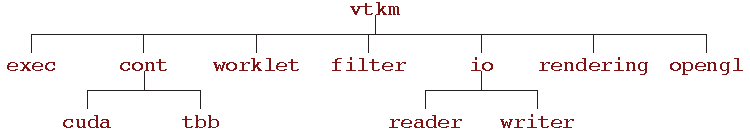
\includegraphics{images/PackageHierarchy}
  \fix{Make a graphic of the package hierarchy.}
  \caption{VTK-m package hierarchy.}
  \label{fig:Packages}
\end{figure}

By convention all classes will be defined in a file with the same name as
the class name (with a \textfilename{.h} extension) located in a directory
corresponding to the package name. For example, the \vtkmcont{ArrayHandle}
class is found in the \vtkmheader{vtkm/cont}{ArrayHandle.h} header. There
are, however, exceptions to this rule. Some smaller classes and types are
grouped together for convenience. These exceptions will be noted as
necessary.

Within each namespace there may also
be \textnamespace{internal}\indexnamespaceone{internal}
and \textnamespace{detail}\indexnamespaceone{detail}
sub-namespaces. The \textnamespace{internal} namespaces contain features
that are used internally and may change without
notice. The \textnamespace{detail} namespaces contain features that are
used by a particular class but must be declared outside of that
class. Users should generally ignore classes in these namespaces.

\index{packages|)}


\section{Function and Method Exports}
\label{sec:FunctionAndMethodExports}

Any function or method defined by VTK-m must come with an export modifier
that determines in which environments the function may be run. These export
modifiers are C macros that VTK-m uses to instruct the compiler for which
architectures to compile each method. Most user code outside of VTK-m need
not use these macros with the important exception of any classes passed to
VTK-m. This occurs when defining new worklets, array containers, and device
adapters.

VTK-m provides three export macros, \vtkmcontexport, \vtkmexecexport, and
\vtkmexeccontexport, which are used to declare functions and methods that
can run in the control environment, export environment, and both
environments, respectively. These macros get defined by including just
about any VTK-m header file, but including \vtkmheader{vtkm}{Types.h} will
ensure they are defined. 

The export macro is place after the template declaration, if there is one,
and before the return type for the function. Here is a simple example of a
function that will square a value. Since most types you would use this
function on have operators in both the control and execution environments,
the function is exported to both places.

\vtkmlisting{Usage of export macro.}{ExportMacro.cxx}

The primary function of the export macros is to interject compiler-specific
keywords that specify what architecture to compile code for. For example,
when compiling with CUDA\index{CUDA}, the control exports have
\textcode{\_\_host\_\_} in them and execution exports have
\textcode{\_\_device\_\_} in them.

There is one additional export macro that is not used for functions but
rather used when declaring a constant data object that is used in the
execution environment. This macro is named
\vtkmmacro{VTKM\_EXEC\_CONSTANT\_EXPORT}\index{export!constant}\index{constant~export}
and is used to declare a constant lookup table used when executing a
worklet. Its primary reason for existing is to add a
\textcode{\_\_constant\_\_} keyword when compiling with CUDA. This export
currently has no effect on any other compiler.


\section{Core Data Types}
\label{sec:CoreDataTypes}

Except in rare circumstances where precision is not a concern, VTK-m does
not directly use the core C types like \textcode{int}, \textcode{float},
and \textcode{double}. Instead, VTK-m provides its own core types, which
are declared in \vtkmheader{vtkm}{Types.h}.

\subsection{Single Number Types}

All floating point values should be declared as type \vtkm{Scalar}, and all
integer values, generally used for indexing, should be declared as type
\vtkm{Id}. The chief advantage of using these declared types rather than
the core C types is that the precision can easily be changed. By default,
both types are 32 bits wide. The CMake configuration options
\cmakevar{VTKM\_USE\_DOUBLE\_PRECISION} and
\cmakevar{VTKM\_USE\_64BIT\_IDS} can be used to change the \vtkm{Scalar}
type and \vtkm{Id} type, respectively, to be 64 bits wide. The
configuration can be overridden by defining the C macro
\vtkmmacro{VTKM\_USE\_DOUBLE\_PRECISION} or
\vtkmmacro{VTKM\_NO\_DOUBLE\_PRECISION} to force \vtkm{Scalar} to be either
64 or 32 bits and defining the C macro \vtkmmacro{VTKM\_USE\_64BIT\_IDS} or
\vtkmmacro{VTKM\_NO\_64BIT\_IDS} to force \vtkm{Id} to be either 64 or 32
bits. These macros must be defined before any VTK-m header files are
included to take effect. For convenience, you can include either
\vtkmheader{vtkm/internal}{ConfigureFor32.h} or
\vtkmheader{vtkm/internal}{ConfigureFor64.h} to force both \vtkm{Scalar}
and \vtkm{Id} to be 32 or 64 bits. The reason VTK-m uses macros to
determine these type widths rather than templates is to reduce the number
of template parameters required in the already template-heavy VTK-m classes
and functions.

\subsection{Vector Types}

Visualization algorithms also often require operations on short vectors.
Arrays indexed in up to three dimensions are common. Data are often defined
in 2-space and 3-space, and transformations are typically done in
homogeneous coordinates of length 4. To simplify these types of operations,
VTK-m provides several vector data types.

The types \vtkm{Id2} and \vtkm{Id3} are couple and triple values of type
\vtkm{Id}. The types \vtkm{Vector2}, \vtkm{Vector3}, and \vtkm{Vector4} are
couple, triple, and quadruple values of type \vtkm{Scalar}. The elements of
these vectors are accessed with the bracket operator, so they syntactically
appear like short arrays. They additionally have a constant named
\textidentifier{NUM\_COMPONENTS}\index{NUM\_COMPONENTS} to specify how many
components are in the tuple.

The default constructor of these vector types leaves the values
uninitialized. All vectors have a constructor with one arguments that is
used to initialize all components. All these vectors also have a
constructor that allows you to set the individual components. Likewise,
there are a set of \vtkm{make\_Id*} and \vtkm{make\_Vector*} functions that
build initialized vector types. \fix{I'm starting to question why we have
  make\_Vector* and make\_Id* when the constructors work just fine. The
  real point of these make* functions is to return a templated type without
  having to declare the template. But none of these methods are templated.}

\vtkmlisting{Creating vector types.}{CreatingVectorTypes.cxx}

The vector types all support component-wise arithmetic using the operators
for plus (\textcode{+}), minus (\textcode{-}), multiply (\textcode{*}), and
divide (\textcode{/}). They also support scalar to vector multiplication
with the multiply operator. The comparison operators equal (\textcode{==})
is true if every pair of corresponding components are true and not equal
(\textcode{!=}) is true otherwise.  A special \vtkm{dot} function is
overloaded to provide a dot product for every type of vector.

\vtkmlisting{Vector operations.}{VectorOperations.cxx}

\subsection{Tuple}

VTK-m provides the templated class \vtkm{Tuple}\tparams{T,Size}, which is
essentially a fixed length array of a given type. \vtkm{Tuple} objects
behave just like the vector types previously described but with any type
and length that you specify.

\vtkmlisting{The tuple class.}{TupleClass.cxx}

The same operators that work on the vector types work on \vtkm{Tuple} with
the caveat that the operator must work on the component type of the
tuple. For example, the multiply operator will work fine on objects of type
\vtkm{Tuple}\tparams{char,3}, but the multiply operator will not work on objects
of type \vtkm{Tuple}\tparams{std::string,3} because you cannot multiply
objects of type \textcode{std::string}.

A \vtkm{Tuple} of the appropriate type can be used interchangeably with a
matching vector type. In fact, a vector type is really just a typedef over
a \vtkm{Tuple}. This is convenient for a number of things including writing
generic functions that work over all types.

\vtkmlisting{Interchangeability of tuples and vector types.}{TuplesAndVectors.cxx}

In addition to generalizing vector operations and making arbitrarily long
vectors, \vtkm{Tuple} is useful for creating any sequence of homogeneous
objects. Here is a simple example of using \vtkm{Tuple} to hold the state of
a polygon.

\vtkmlisting{Usage of a tuple.}{EquilateralTriangle.cxx}

\subsection{Extents}

\vtkm{Extent3} is a simple structure that holds the extent information for
structured data (data defined on a regular grid). It contains two
\vtkm{Id3} fields named \textcode{Min} and \textcode{Max} that define the
minimum and maximum 3D index. \textcode{Min} and \textcode{Max} are
\emph{inclusive} point indices.

Although less used, there also exists \vtkm{Extent2}, which is the same as
\vtkm{Extent3} except for structured grids with 2 topological
dimensions. The two structures are exactly the same except that
\vtkm{Extent2} uses \vtkm{Id2} objects for its \textcode{Min} and
\textcode{Max} instead of \vtkm{Id3}. There is also a generic structure
named \vtkm{Extent} that takes a single integer argument to make the
structured extent for some arbitrary topological dimension.

\vtkm{Extent3} and the other extent structures are defined in the
\vtkmheader{vtkm}{Extent.h} header. This header also contains the following
helper functions.

\begin{description}
\item[\vtkm{ExtentPointDimensions}] Takes an extent object as an argument
  and returns a \vtkm{Id3} (or other appropriately sized tuple) giving the
  number of points in each topological dimension.
\item[\vtkm{ExtentCellDimensions}] Takes an extent object as an argument
  and returns a \vtkm{Id3} (or other appropriately sized tuple) giving the
  number of cells in each topological dimension. The number of cells is one
  less than the number of points in each dimensions.
\item[\vtkm{ExtentNumberOfPoints}] Takes an extent object as an argument
  and returns the number of points in an associated structured mesh.
\item[\vtkm{ExtentNumberOfCells}] Takes an extent object as an argument and
  returns the number of cells in an associated structured mesh.
\item[\vtkm{ExtentPointFlatIndexToTopologyIndex}] Elements in structured
  grids have a single index with 0 being the entry at the minimum extent in
  every direction and then increasing first in the $r$ direction, then the
  $s$ direction, and then the $t$ direction. This function takes a flat
  point index as its first argument and an extent as its second argument
  and returns the ${r,s,t}$ topological coordinates in a \vtkm{Id3} (or
  other appropriately sized tuple).
\item[\vtkm{ExtentCellFlatIndexToTopologyIndex}] Takes a flat cell index as
  its first argument and an extent as its second argument and returns the
  ${r,s,t}$ topological coordinates in a \vtkm{Id3} (or other appropriately
  sized tuple).
\item[\vtkm{ExtentPointTopologyIndexToFlatIndex}] Takes topological point
  coordinates as the first argument and an extent as the second argument
  and returns the equivalent flat point index.
\item[\vtkm{ExtentCellTopologyIndexToFlatIndex}] Takes topological cell
  coordinates as the first argument and an extent as the second argument
  and returns the equivalent flat cell index.
\item[\vtkm{ExtentFirstPointOnCell}] Takes a flat cell index as its first
  argument and returns the flat index to the first point incident on that
  cell. This is a convenience function for some operations that relate
  cells to points.
\end{description}

The following example demonstrates using a \vtkm{Extent3} and the
supporting functions. Extents of different dimensions work
corredspondingly.

\vtkmlisting{Creating and using an \textidentifier{Extent3}.}{Extent3.cxx}

\subsection{Pair}

\fix{Pair not implemented yet. (Maybe it won't be.)}

%% VTK-m defines a \vtkm{Pair}\tparams{T1,T2} templated object that
%% behaves just like \textcode{std:\colonhyp{}pair} from the standard template
%% library. The difference is that \vtkm{Pair} will work in both the execution
%% and control environment, whereas the STL \textcode{std::pair} does not
%% always work in the execution environment.

%% The VTK-m version of \vtkm{Pair} supports the same types, fields, and
%% operations as the STL version. VTK-m also provides a \vtkm{make\_Pair}
%% function for convenience.

\section{Traits}
\label{sec:Traits}

\index{traits|(}

When using templated types, it is often necessary to get information about
the type or specialize code based on general properties of the type. VTK-m
uses traits classes to publish and retrieve information about types. A
traits class is simply a templated structure that provides typedefs for
tag\index{tag} structures, empty types used for identification. The traits
classes might also contain constant numbers and helpful static
functions. See {\it Effective C++ Third Edition} by Scott Mayers for a
description of traits classes and their uses.

\subsection{Type Traits}

The \vtkm{TypeTraits}\tparams{T} templated class provides basic information
about a core type. These type traits are available for all the basic C++
types as well as the core VTK-m types described in
Section~\ref{sec:CoreDataTypes}. \vtkm{TypeTraits} contains the following
elements.

\index{tag!type traits|(}

\begin{description}
\item[\textidentifier{NumericTag}] \index{NumericTag} \index{tag!numeric}
  This type is set to either \vtkm{TypeTraitsRealTag} or
  \vtkm{TypeTraitsIntegerTag} to signal that the type represents either
  floating point numbers or integers.
\item[\textidentifier{DimensionalityTag}] \index{DimensionalityTag}
  \index{tag!dimensionality} This type is set to either
  \vtkm{TypeTraitsScalarTag} or \vtkm{TypeTraitsVectorTag} to signal that
  the type represents either a single scalar value or a tuple of values.
\end{description}

The definition of \vtkm{TypeTraits} for \vtkm{Scalar} could like something
like this.
\begin{vtkmexample}{Definition of \protect \vtkm{TypeTraits}\tparams{\protect \vtkm{Scalar}}.}
namespace vtkm {

template<>
struct TypeTraits<vtkm::Scalar>
{
  typedef vtkm::TypeTraitsRealTag NumericTag;
  typedef vtkm::TypeTraitsScalarTag DimensionalityTag;
};

}
\end{vtkmexample}

Here is a simple example of using \vtkm{TypeTraits} to implement a generic
function that behaves like the remainder operator (\textcode{\%}) for all
types including floating points and vectors.

\fix{The following example uses the POSIX math floor function. It should be
  replaced with the VTK-m version of floor when available.}

\vtkmlisting[ex:TypeTraits]{Using \textidentifier{TypeTraits} for a generic remainder.}{TypeTraits.cxx}

\index{tag!type traits|)}


\subsection{Vector Traits}

The \vtkm{VectorTraits}\tparams{T} templated class provides information and
accessors to vector and tuple types. It contains the following elements.

\index{tag!vector traits|(}

\begin{description}
\item[\textidentifier{ComponentType}] \index{ComponentType} This type is
  set to the type for each component in the vector. For example, a
  \vtkm{Vector3} has \textidentifier{ComponentType} defined as
  \vtkm{Scalar}.
\item[\textidentifier{NUM\_COMPONENTS}] \index{NUM\_COMPONENTS} An integer
  specifying how many components are contained in the vector.
\item[\textidentifier{HasMultipleComponents}] \index{HasMultipleComponents}
  \index{tag!single component} \index{tag!multiple components}
  This type is set to either \vtkm{VectorTraitsTagSingleComponent} if the
  vector length is size 1 or \vtkm{VectorTraitsTagMultipleComponents}
  otherwise. This tag can be useful for creating specialized functions when
  a vector is really just a scalar.
\item[\textcode{GetComponent}] \index{GetComponent} A static method that
  takes a vector and returns a particular component.
\item[\textcode{SetComponent}] \index{SetComponent} A static method that
  takes a vector and sets a particular component to a given value.
\item[\textcode{ToTuple}] \index{ToTuple} A static method that converts a
  vector of the given type to a \vtkm{Tuple}.
\end{description}

The definition of \vtkm{VectorTraits} for \vtkm{Id3} could like something
like this.
\begin{vtkmexample}{Definition of \protect \vtkm{VectorTraits}\tparams{\protect \vtkm{Id3}}.}
namespace vtkm {

template<>
struct VectorTraits<vtkm::Id3>
{
  typedef vtkm::Id ComponentType;
  static const int NUM_COMPONENTS = 3;
  typedef VectorTraitsTagMultipleComponents HasMultipleComponents;

  VTKM_EXEC_CONT_EXPORT
  static vtkm::Id &GetComponent(vtkm::Id3 &vector, int component) {
    return vector[component];
  }

  VTKM_EXEC_CONT_EXPORT
  static void SetComponent(vtkm::Id3 &vector, int component, vtkm::Id value) {
    vector[component] = value;
  }

  VTKM_EXEC_CONT_EXPORT
  static vtkm::Tuple<vtkm::Id,3> ToTuple(const vtkm::Id3 &vector) {
    return vector;
  }
};

} // namespace vtkm
\end{vtkmexample}

\index{tag!vector traits|)}

The real power of vector traits is that they simplify creating generic
operations on any type that can look like a vector. This includes
operations on scalar values as if they were vectors of size one. The
following code uses vector traits to simplify the implementation of less
functors\index{less} that define an ordering that can be used for sorting
and other operations.

\vtkmlisting{Using \textidentifier{VectorTraits} for less functors.}{VectorTraits.cxx}

\index{traits|)}


\section{List Tags}
\label{sec:ListTags}

\index{tag!lists|(}
\index{lists|(}

\index{template metaprogramming}
\index{metaprogramming}
VTK-m internally uses template metaprogramming, which utilizes the C++
template to run source-generating programs, to customize code to various
data and compute platforms. One basic structure often uses with template
metaprogramming is a list of class names (also sometimes called a tuple or
vector, although both of those names have different meanings in VTK-m).

Many VTK-m users only need predefined lists, such as the type lists
specified in Section~\ref{sec:TypeLists} or the container lists specified
in Section~\ref{sec:ContainerLists}. Those users can skip most of the
details of this section. However, it is sometimes useful to modify lists,
create new lists, or operate on lists, and these usages are documented
here.

VTK-m uses a tag-based mechanism for defining lists, which differs
significantly from lists in many other template metaprogramming libraries
such as with \textcode{boost:\colonhyp{}mpl:\colonhyp{}vector} or
\textcode{boost:\colonhyp{}vector}. Rather than enumerating all list
entries as template arguments, the list is referenced by a single tag class
with a descriptive name. The intention is to make fully resolved types
shorter and more readable. (Anyone experienced with template programming
knows how insanely long and unreadable types can get in compiler errors and
warnings.)

\subsection{Building List Tags}
\label{sec:BuildingListTags}

List tags are constructed in VTK-m by defining a \textcode{struct} that
publicly inherits from another list tags. The base list tags are defined in
the \vtkmheader{vtkm}{ListTag.h} header.

The most basic list is defined with \vtkm{ListTagEmpty}. This tag
represents an empty list.

\vtkm{ListTagBase}\tparams{T} represents a list of size one containing the
class named in the template parameter. The tags
\vtkm{ListTagBase2}\tparams{T1,T2}, \vtkm{ListTagBase3}\tparams{T1,T2,T3},
and \vtkm{ListTagBase4}\tparams{T1,T2,T3,T4} provide convenient ways to
define lists with up to 4 items.

Finally, lists can be combined together with
\vtkm{ListTagJoin}\tparams{ListTag1,ListTag2}, which concatinates two lists
together.

The following example demonstrates how to build list tags using these base
lists classes. Note first that all the list tags are defined as
\textcode{struct} rather than \textcode{class}. Although these are roughly
synonymous in C++, \textcode{struct} inheritance is by default public, and
public inheritance is important for the list tags to work. Note second that
these tags are created by inheritance rather than using
\textcode{typedef}. Although \textcode{typedef} will work, it will lead to
much uglier type names defined by the compiler.

\vtkmlisting{Creating list tags.}{BaseListTags.cxx}

\subsection{Type Lists}
\label{sec:TypeLists}

\index{type lists|(}
\index{lists!types|(}
\index{tag!type lists|(}

One of the major use cases for template metaprogramming lists in VTK-m is
to identify a set of potential data types for arrays. The
\vtkmheader{vtkm}{TypeListTag.h} header contains predefined lists for known
VTK-m types. Although technically all these lists are of C++ types, the
types we refer to here are those data types stored in data arrays.

There is a list tag for a list containing a single type for every data type
defined by VTK-m. These tags are: \vtkm{TypeListTagId},
\vtkm{TypeListTagId2}, \vtkm{TypeListTagId3}, \vtkm{TypeListTagScalar},
\vtkm{TypeListTagVector2}, \vtkm{TypeListTagVector3}, and
\vtkm{TypeListTagVector4}.

\vtkm{TypeListTagAll} is a list tag containing all the basic types in
VTK-m. It is a concatenation of all the types listed in the previous
paragraph.

\vtkm{TypeListTagIndex} is a list of all the types appropriate for
indices. Specifically, it contains the types \vtkm{Id}, \vtkm{Id2},
\vtkm{Id3}. \vtkm{TypeListTagReal} is a list of all the types for floating
point numbers. Specifically, it contains the types \vtkm{Scalar},
\vtkm{Vector2}, \vtkm{Vector3}, \vtkm{Vector4}.

\vtkm{TypeListTagCommon} is a list of the most commonly used types across
multiple domains. It contains the types \vtkm{Id}, \vtkm{Scalar},
\vtkm{Vector3}.

If these lists are not sufficient, it is possible to build new type lists
using the existing type lists and the list bases from
Section~\ref{sec:BuildingListTags} as demonstrated in the following
example.

\vtkmlisting[ex:CustomTypeLists]{Defining new type lists.}{CustomTypeLists.cxx}

The \vtkmheader{vtkm}{TypeListTag.h} header also defines a macro named
\vtkmmacro{VTKM\_DEFAULT\_TYPE\_LIST\_TAG} that defines a default list of
types to use in classes like \vtkmcont{DynamicArrayHandle}
(Section~\ref{sec:DynamicArrayHandle}). This list can be overridden by
defining the \vtkmmacro{VTKM\_DEFAULT\_TYPE\_LIST\_TAG} macro \emph{before}
any VTK-m headers are included. If included after a VTK-m header, the list
is not likely to take effect. Do not ignore compiler warnings about the
macro being redefined, which you will not get if defined
correctly. Example~\ref{ex:CustomTypeLists} also contains an example of
overriding the \vtkmmacro{VTKM\_DEFAULT\_TYPE\_LIST\_TAG} macro.

\index{tag!type lists|)}
\index{lists!types|)}
\index{type lists|)}

\subsection{Operating on Lists}
\label{sec:OperatingOnLists}

VTK-m template metaprogramming lists are typically just passed to VTK-m
methods that internally operate on the lists. Although not typically used
outside of the VTK-m library, these operations are also available.

The \vtkmheader{vtkm}{ListTag.h} header comes with a \vtkm{ListForEach}
function that takes a functor object and a list tag. It then calls the
functor object with the default object of each type in the list. This is
most typically used with C++ run-time type information to convert a
run-time polymorphic object to a statically typed (and possibly inlined)
call.

The following example shows a rudimentary version of coverting a
dynamically-typed array to a statically-typed array similar to what is done
in VTK-m classes like \vtkmcont{DynamicArrayHandle} (which is documented in
Section~\ref{sec:DynamicArrayHandle}).

\vtkmlisting{Converting dynamic types to static types with \textidentifier{ListForEach}.}{ListForEach.cxx}

\index{lists|)}
\index{tag!lists|)}
